\section{Durchführung}
\label{sec:Durchführung}

\subsection{Untersuchungen am Zählrohr}

Die Anordnung sieht wie in Abb. \ref{fig:aufbau} dargestellt aus. Durch die gesammelten Ladungen $Q$ entsteht ein messbarer Spannungsimpuls. Dieser wird über den Kondensator ausgekoppelt und nach der Verstärkung im Zählgerät registriert.
%Außerdem wird der Eingang auf dem Oszilloskop angezeigt.

\begin{figure}
    \centering
    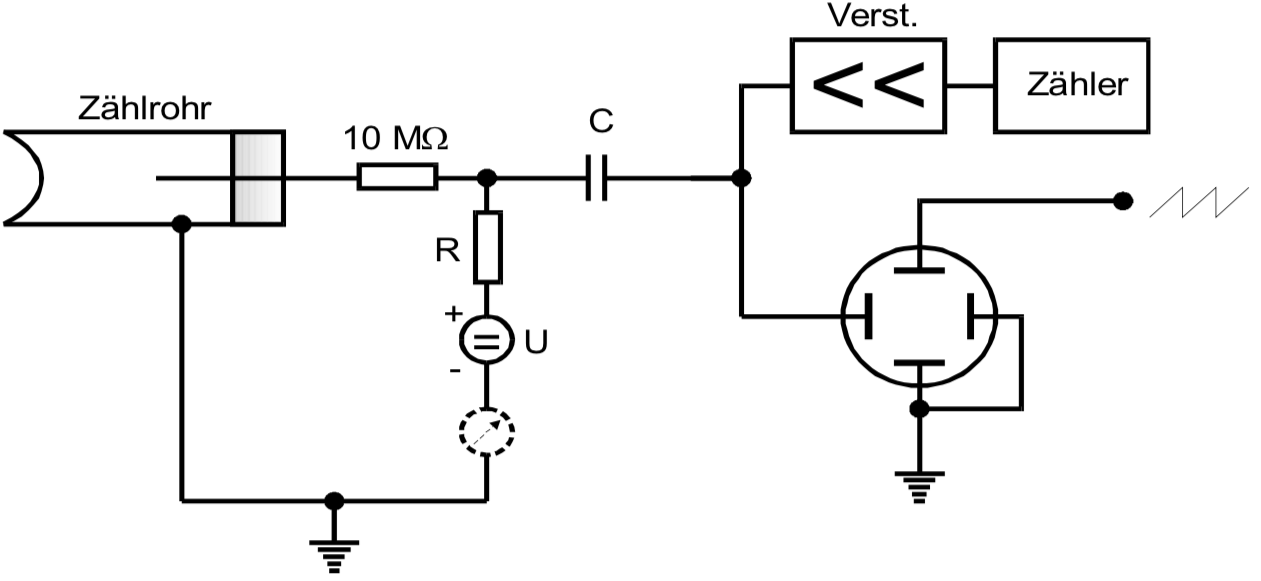
\includegraphics[width=12cm, height=6cm]{build/aufbau.png}
    \caption{Zu sehen ist der Aufbau der Apparatur. Das Zählrohr ist an einer Spannungsquelle angeschlossen. Der Strom kann durch ein Mikroamperemeter gemessen werden. Außerdem sind ein Verstärker und ein Zähler angeschlossen. \cite{V703}}
    \label{fig:aufbau}
\end{figure}

\subsection{Messung der Charakteristik}
Eine \beta-Quelle wird vor das Zählrohr gestellt und die Zählrate wird in Abhängigkeit von der Betriebsspannung $U$ gemessen. Dabei wird zwischen Quelle und Zählrohr ein Stück Papier gestellt, um die Strahlungsintensität zu schwächen.

\noindent Die Spannung wird zunächst auf $\SI{320}{\volt}$ gestellt und in $\SI{20}{\volt}$ Schritten auf $\SI{680}{\volt}$ erhöht.

\noindent Mithilfe eines Strommessgeräts wird dabei der mittlere Zählrohrstrom gemessen.


\subsection{Messung der Totzeit}
\subsubsection{Messung mit dem Oszillographen}
Die Strahlintensität wird wieder erhöht, indem das Papier entfernt wird.
Die Spannung wird auf $\SI{500}{\volt}$ gestellt, damit die Messung etwa in der Mitte des Plateaus stattfindet.
Die Zeitablenkung des Oszillographen wird durch die Anstiegsflanke getriggert, sodass die Totzeit abgelesen werden kann. Diese entspricht dabei der Strecke auf der $x$-Achse, die mit dem Anfang der Kurve beginnt und bei dem gedachten Schnitt der ersten Nachentladungskurve mit der Achse endet (siehe Abb. \ref{fig:totzeit}).

\subsubsection{Messung mit der Zwei-Quellen-Methode}
Es wird die Totzeit mit der Zwei-Quellen-Methode gemessen. Dafür wird bei einer Spannung von $\SI{500}{V}$ die Anzahl der registrierten Teilchen pro $\SI{60}{\second}$ des ersten Präparats gemessen. Anschließend wird ein zweites Präparat hinzugefügt. Die Zählrate wird wieder gemessen. Zum Schluss wird das erste Präparat entfernt und die Zählrate des zweiten Präparats wird gemessen.